\documentclass[landscape]{article}
\usepackage[pdftex]{graphicx,color,rotating}
\usepackage{ulem}
\pagestyle{empty}
\oddsidemargin  -0.5 in
\evensidemargin -0.5 in
\headheight     0 in
\topmargin      -1 in
\textheight     7.7 in
\textwidth      10 in
\begin{document}
\huge
\renewcommand{\labelitemi}{-}
\setlength{\parindent}{0 cm}
\hyphenpenalty=5000
\tolerance=1000

\mbox{ }

\vfill

\begin{center}
  \Huge $\Gamma_{ee}$ Hadronic Efficiency Measurement Completed! \\

  \vspace{1.5 cm}
  Jim Pivarski
\end{center}

\vfill

\mbox{ }

\pagebreak

\mbox{ }

\vfill

Draft CBX: {\tt /nfs/papers/drafts/gamma\_ee\_efficiency.pdf}

\vfill

Technique: need to know hadronic efficiency of 9 cuts (first is trigger)
\begin{itemize}\setlength{\itemsep}{0.5 cm}

  \item Put Monte Carlo through first six cuts, count survivors for
  efficiency; \\ overlay data and estimate systematic errors

  \item Put background-subtracted data through last three, count
  survivors for efficiency

\end{itemize}

\vfill

\begin{center}\renewcommand{\arraystretch}{1.5}
  \begin{tabular}{p{0.28\linewidth} c c c}
    & $\Upsilon(1S)$ & $\Upsilon(2S)$ & $\Upsilon(3S)$ \\\hline
    Cuts \#1 -- \#6 (MC)   & \mbox{ }98.9\% $\pm$ 0.5\% &  97.2 $\pm$ 0.7\% &  98.2\% $\pm$ 0.7\% \\
    Cuts \#7 -- \#9 (data) &        100.1\% $\pm$ 0.2\% &  99.8 $\pm$ 0.3\% &  98.6\% $\pm$ 0.4\% \\\hline\hline
    & \mbox{ }99.1\% $\pm$ 0.6\% &  97.0 $\pm$ 0.8\% &  96.8\% $\pm$ 0.8\% \\
  \end{tabular}
\renewcommand{\arraystretch}{1}\end{center}

\vfill

\mbox{ }

\pagebreak

{\bf Example: Cut \# 6: Visible energy $>$ 35\% of center-of-mass energy}

\vfill

Central value for efficiency comes from the Monte Carlo

\begin{center} but what uncertainty should be assigned? \end{center}

\vfill

Below: background-subtracted data (points) and Monte Carlo (histogram)
for $\Upsilon(2S)$ (cuts \#1 -- \#5 have been applied: leptons,
beam-gas, and cosmic rays are gone)

\vfill

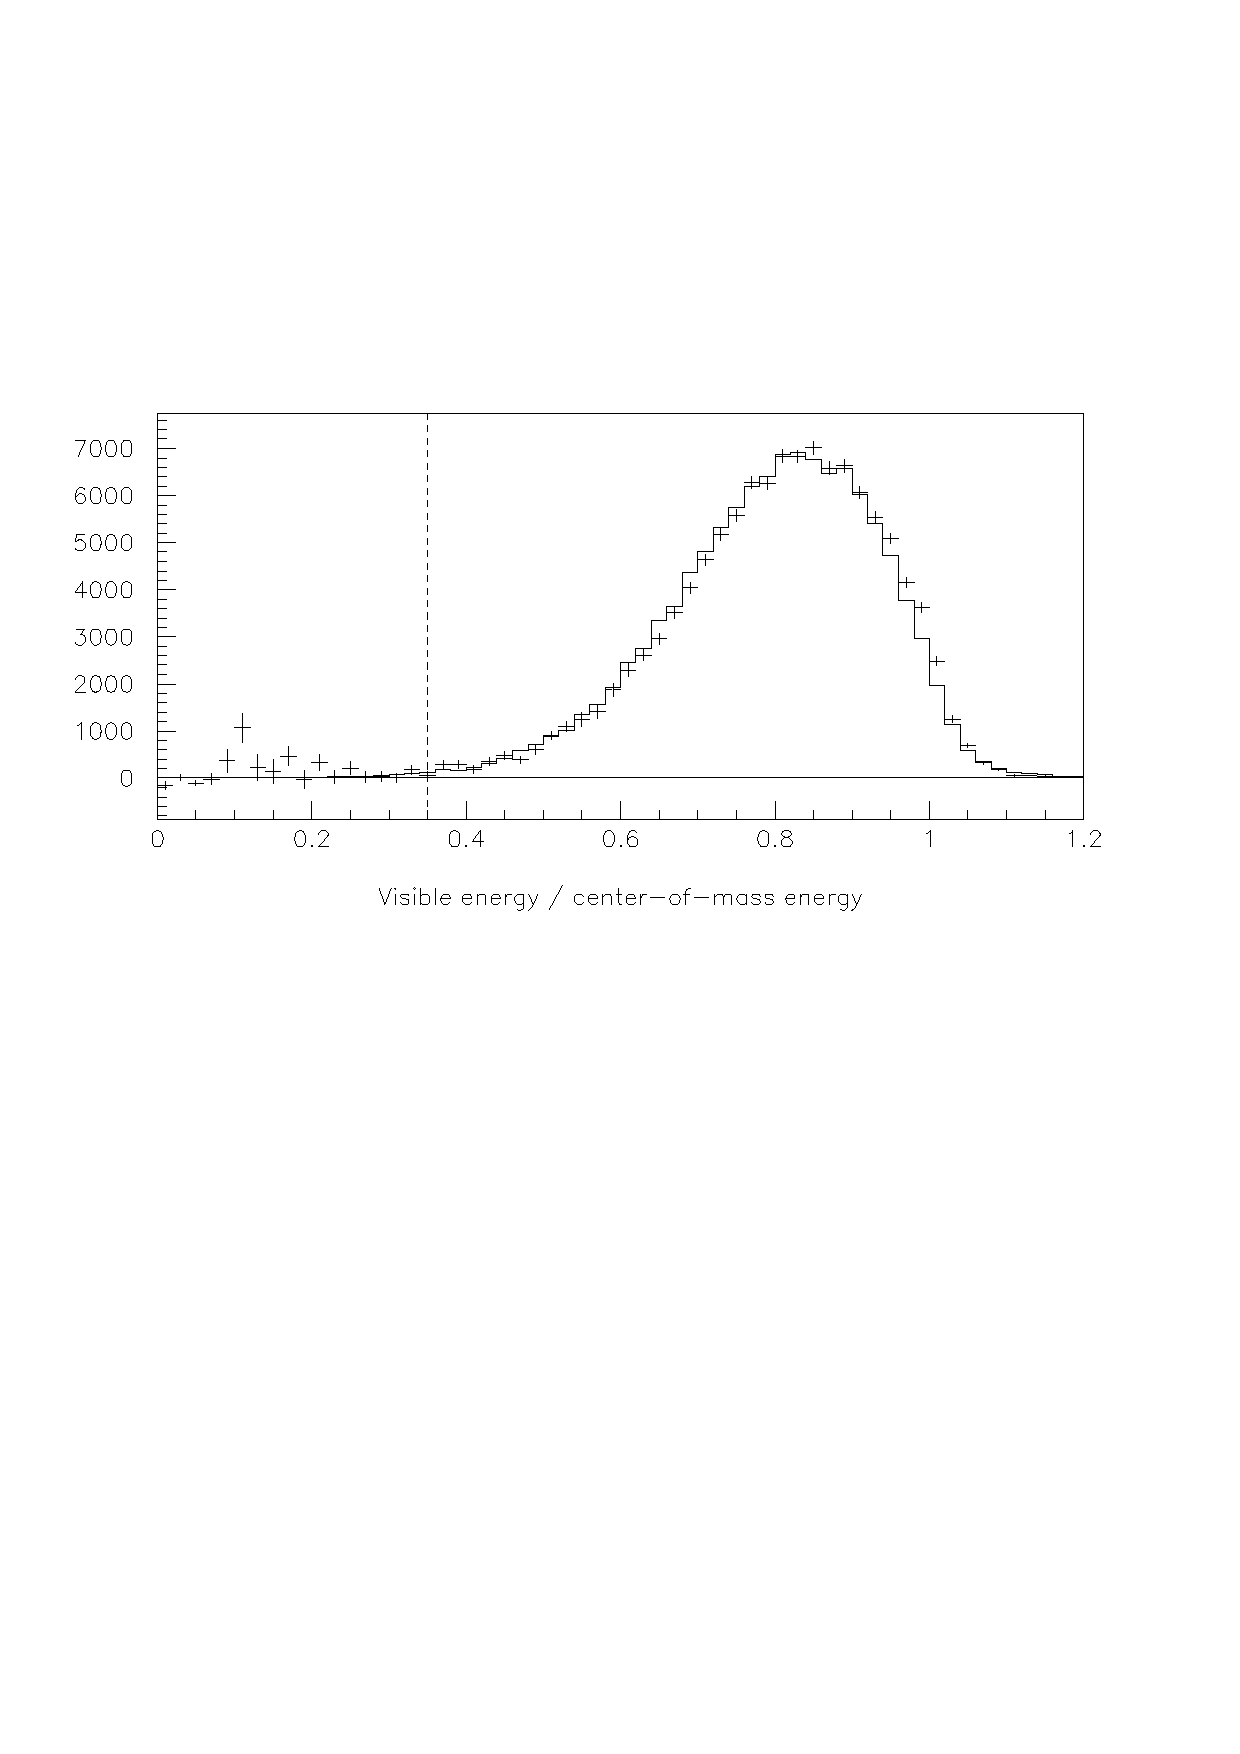
\includegraphics[width=\linewidth]{visen.pdf}

\pagebreak

{\bf Example: Cut \# 6: Visible energy $>$ 35\% of center-of-mass energy}

\vfill

Data before background subtraction has a large peak of mostly
two-photon fusion

\vfill

Continuum scale factor is

\vfill

\[
\frac{\mathcal{L}_{\mbox{\large on-res}}}{\mathcal{L}_{\mbox{\large off-res}}}
\left[\frac{s_{\mbox{\large off-res}}}{s_{\mbox{\large on-res}}} (\mbox{non-$2\gamma$ fraction}) +
\log\left(\frac{s_{\mbox{\large on-res}}}{s_{\mbox{\large off-res}}}\right) (\mbox{$2\gamma$ fraction})\right]
\]

\vfill

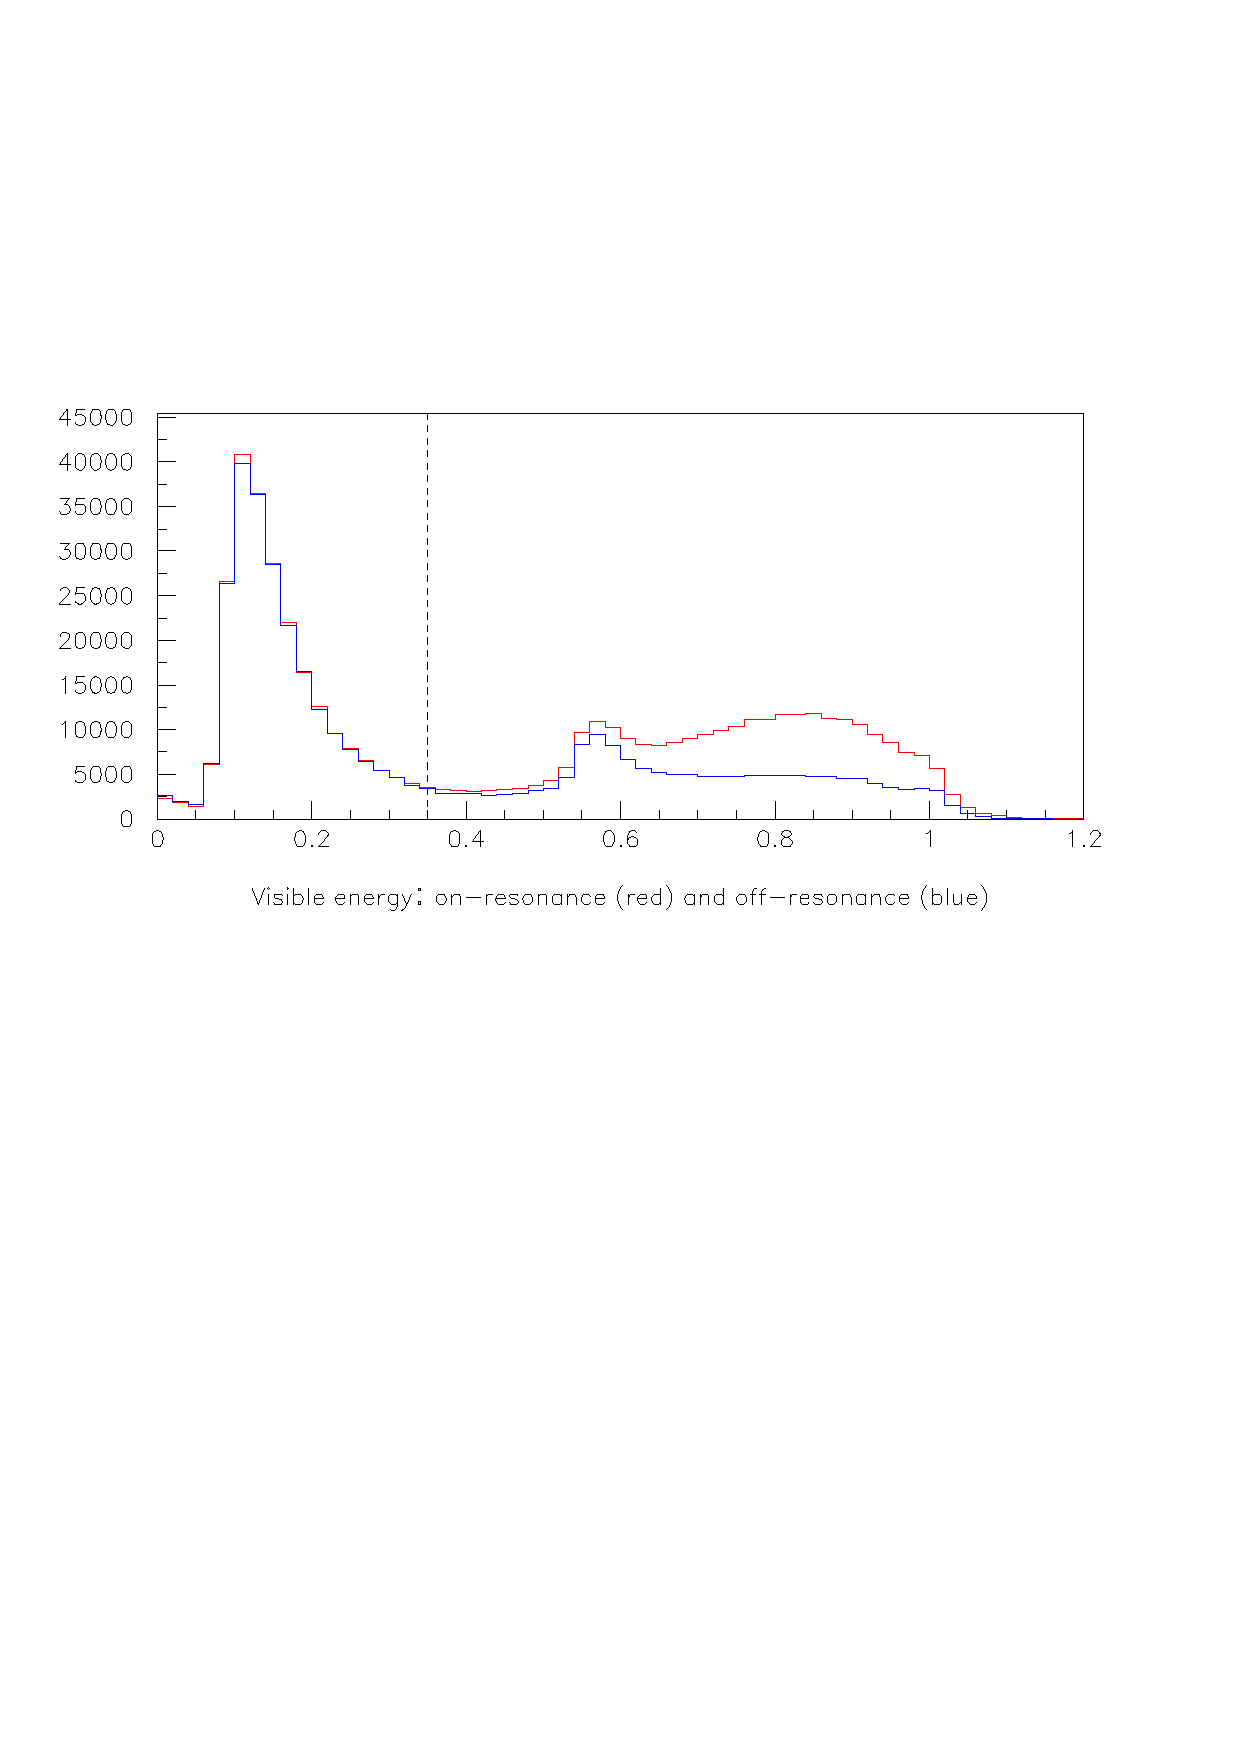
\includegraphics[width=\linewidth]{subtraction.pdf}

\pagebreak

{\bf Example: Cut \# 6: Visible energy $>$ 35\% of center-of-mass energy}

\vfill

Subtraction of large peak {\it and} uncertainty in two-photon fraction
makes data inconclusive at low visible energy.

\vspace{-0.5 cm}
\begin{center}\renewcommand{\arraystretch}{1.2}
  \begin{tabular}{p{0.5\linewidth} c c c}
  & $\varepsilon_{\Upsilon(1S)}$ & $\varepsilon_{\Upsilon(2S)}$ & $\varepsilon_{\Upsilon(3S)}$ \\
  Ignore Monte Carlo, take data uncertainty & $\pm$1.2\% & $\pm$1.5\% & $\pm$2.0\% \\
  Trade assumtions for precision  & $\pm$0.6\% & $\pm$0.8\% & $\pm$0.8\% \\
  \end{tabular}
\renewcommand{\arraystretch}{1}\end{center}

\vfill

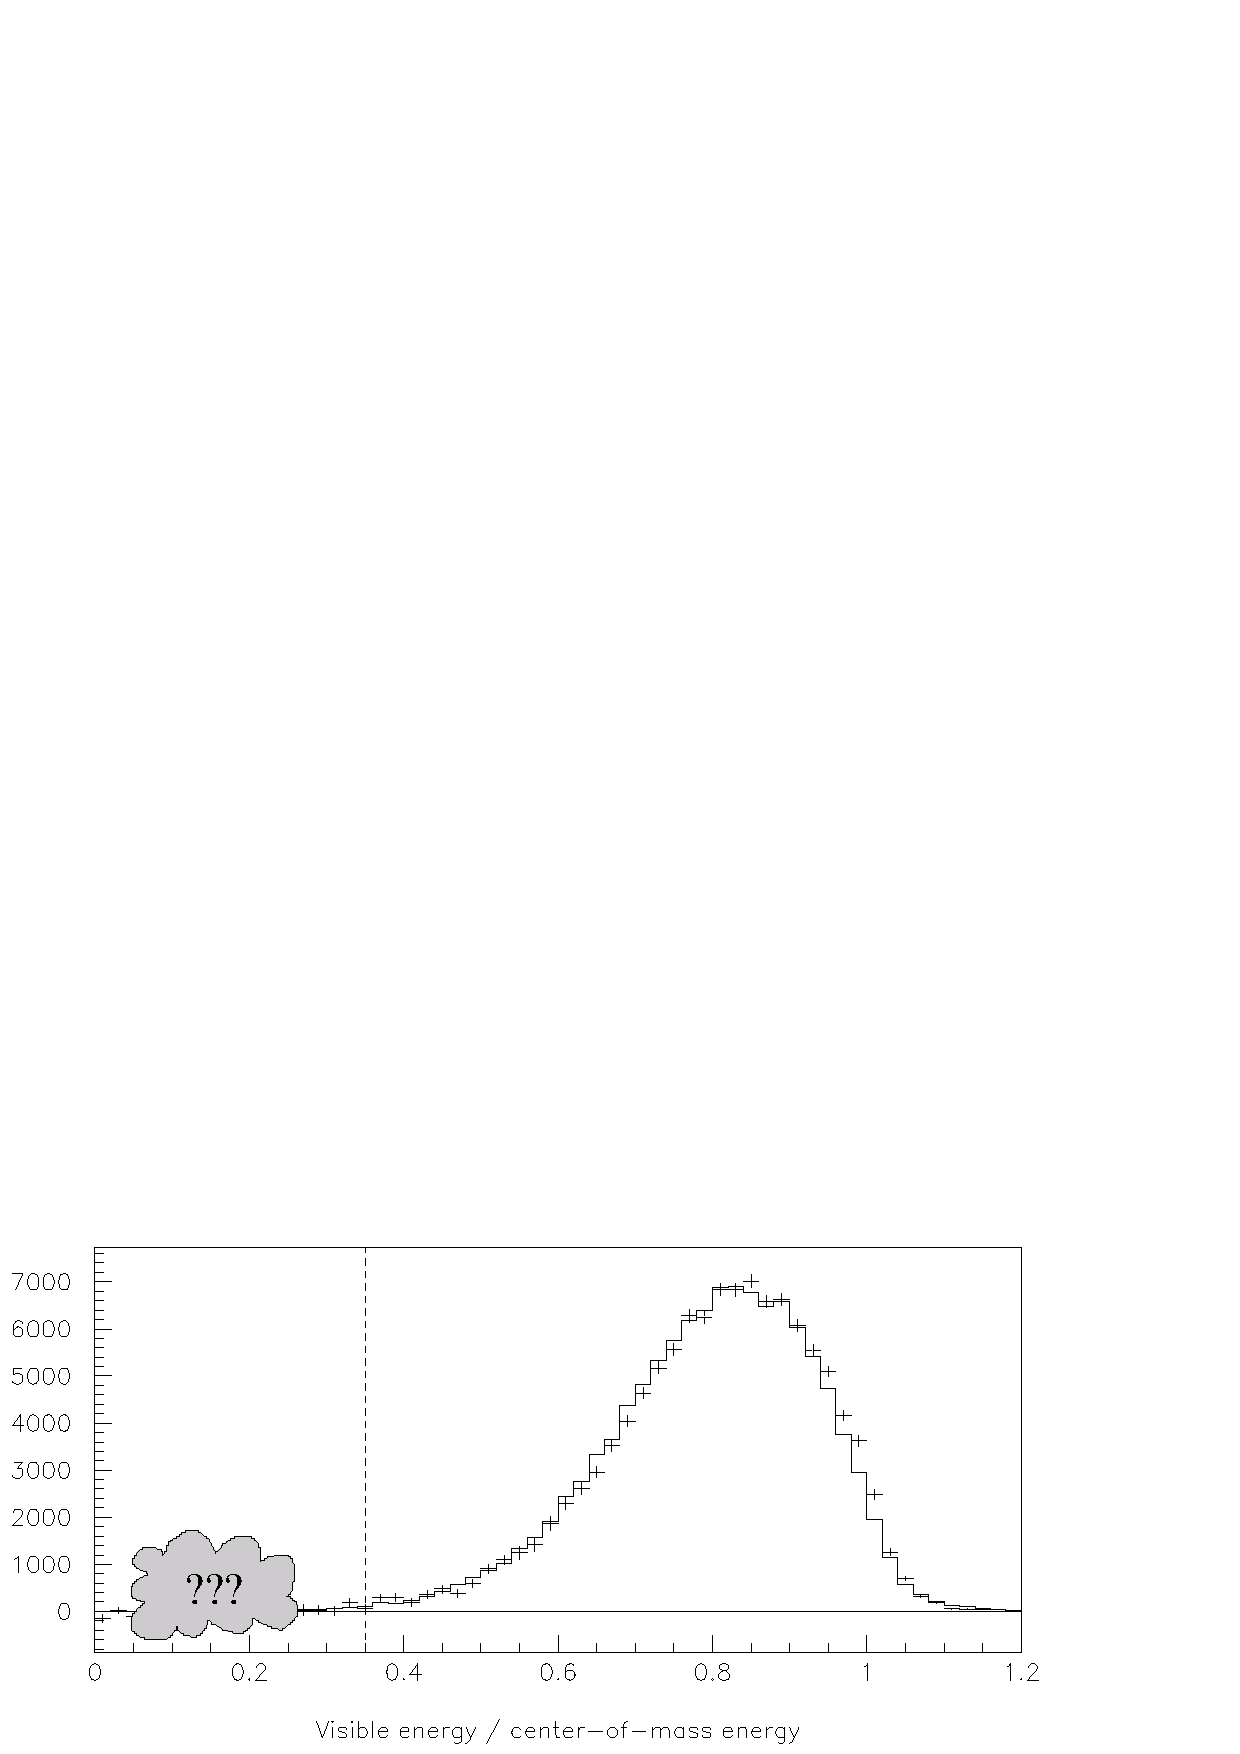
\includegraphics[width=\linewidth]{visen2.pdf}

\pagebreak

{\bf Example: Cut \# 6: Visible energy $>$ 35\% of center-of-mass energy}

\vfill

\begin{center} Why don't I trust Monte Carlo? \end{center}

\vspace{0.5 cm}

\begin{enumerate}\setlength{\itemsep}{0.5 cm}

  \item Explicit decay modes are okay, but real $ggg$, $q\bar{q}$, and
  $gg\gamma$ hadronize via QCD; \\ Monte Carlo approximates with
  Jetset 7.4.

  \item Real $\Upsilon$s might also decay to a final state not in the
  Monte Carlo \\ (given the way I defined my signal, this would be
  signal).

\end{enumerate}

\vfill

\begin{center}\begin{minipage}{0.8\linewidth}

\begin{center} New explicit assumtion (answers objection \#2): \end{center}

\vspace{0.3 cm}

$\Upsilon$s decay only to:

\begin{center}\begin{minipage}{0.9\linewidth}
\begin{itemize}

  \item $ggg$, $q\bar{q}$, and $gg\gamma$, which hadronize (signal)

  \item Cascades to lower $\Upsilon$ with $\pi\pi$ or $\gamma\gamma$ (signal)

  \item Radiative decays to $\chi_b$ (signal)

  \item $e^+e^-(\gamma)$, $\mu^+\mu^-(\gamma)$, and
  $\tau^+\tau^-(\gamma)$ (not signal)

\end{itemize}\end{minipage}\end{center}

\end{minipage}\end{center}

\vfill

\pagebreak

{\bf Example: Cut \# 6: Visible energy $>$ 35\% of center-of-mass energy}

\vfill

What can still go wrong?  (Objection \#1, previous slide)

\vfill

Suppose $\Upsilon$ decays to a final state which {\it usually} has
lots of missing energy, and this final state is enhanced by some QCD
resonance.

\vfill

Monte Carlo sometimes generates the final state, but doesn't enhance
it because Jetset doesn't know about the resonance.

\vfill

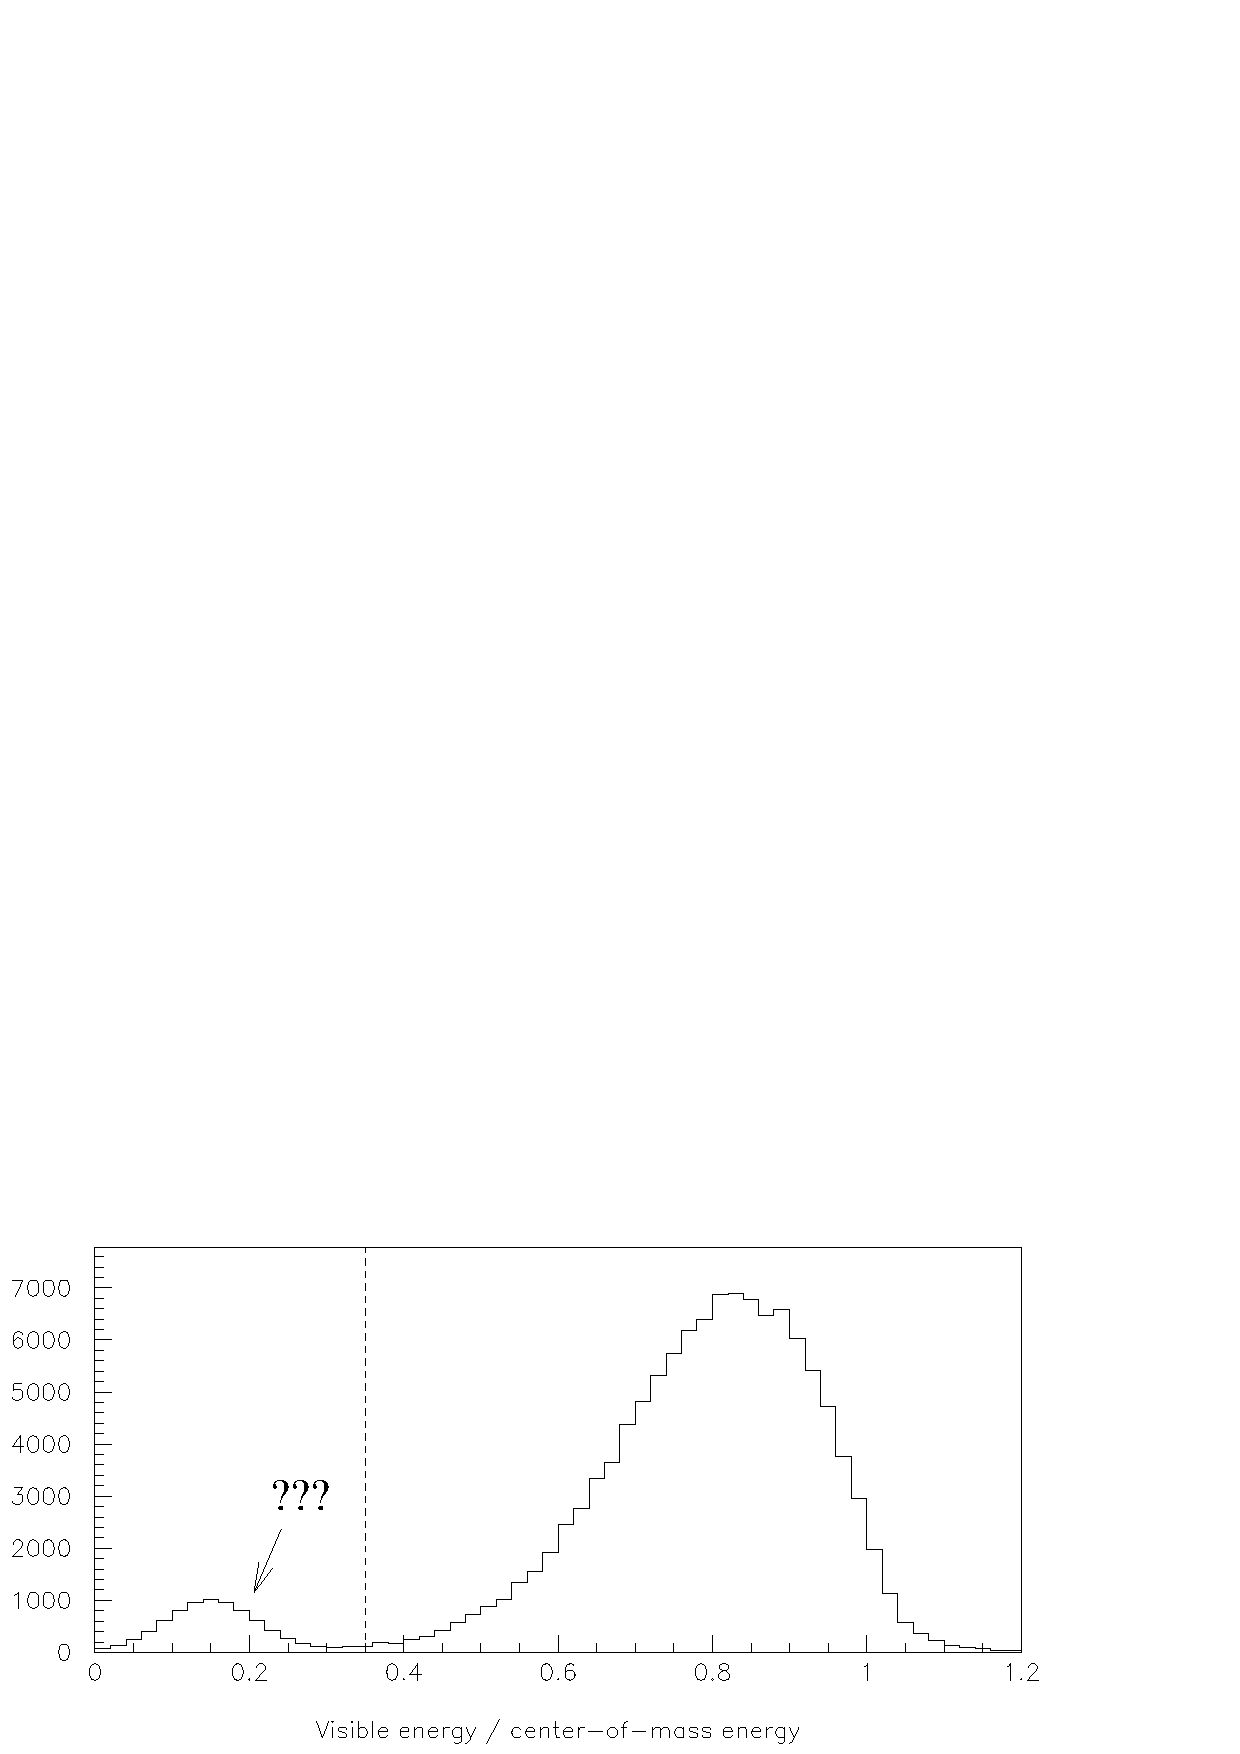
\includegraphics[width=\linewidth]{visen3_revamp.pdf}

\pagebreak

{\bf Example: Cut \# 6: Visible energy $>$ 35\% of center-of-mass energy}

\vfill

Such a final state would most likely be low multiplicity (2- or
3-body) to manage to hide most of its energy most of the time.

\begin{itemize}

  \item Back-to-back down the beamline

  \item Pairs of long-lived strange particles which decay in the detector \\
  (tracks beyond 3 cm are not counted!)
\end{itemize}

\vfill

\includegraphics[width=\linewidth]{versus_multiplicity_revamp.pdf}

\pagebreak

{\bf Example: Cut \# 6: Visible energy $>$ 35\% of center-of-mass energy}

\vfill

Assume it does the most damage possible: 2- and 3-body decays below
threshold are a factor of 10 more common than Monte Carlo thinks.

\vfill

$\Longrightarrow$ Inefficiency of 0.3\% acquires uncertainty bound of 0.2\%

\vfill

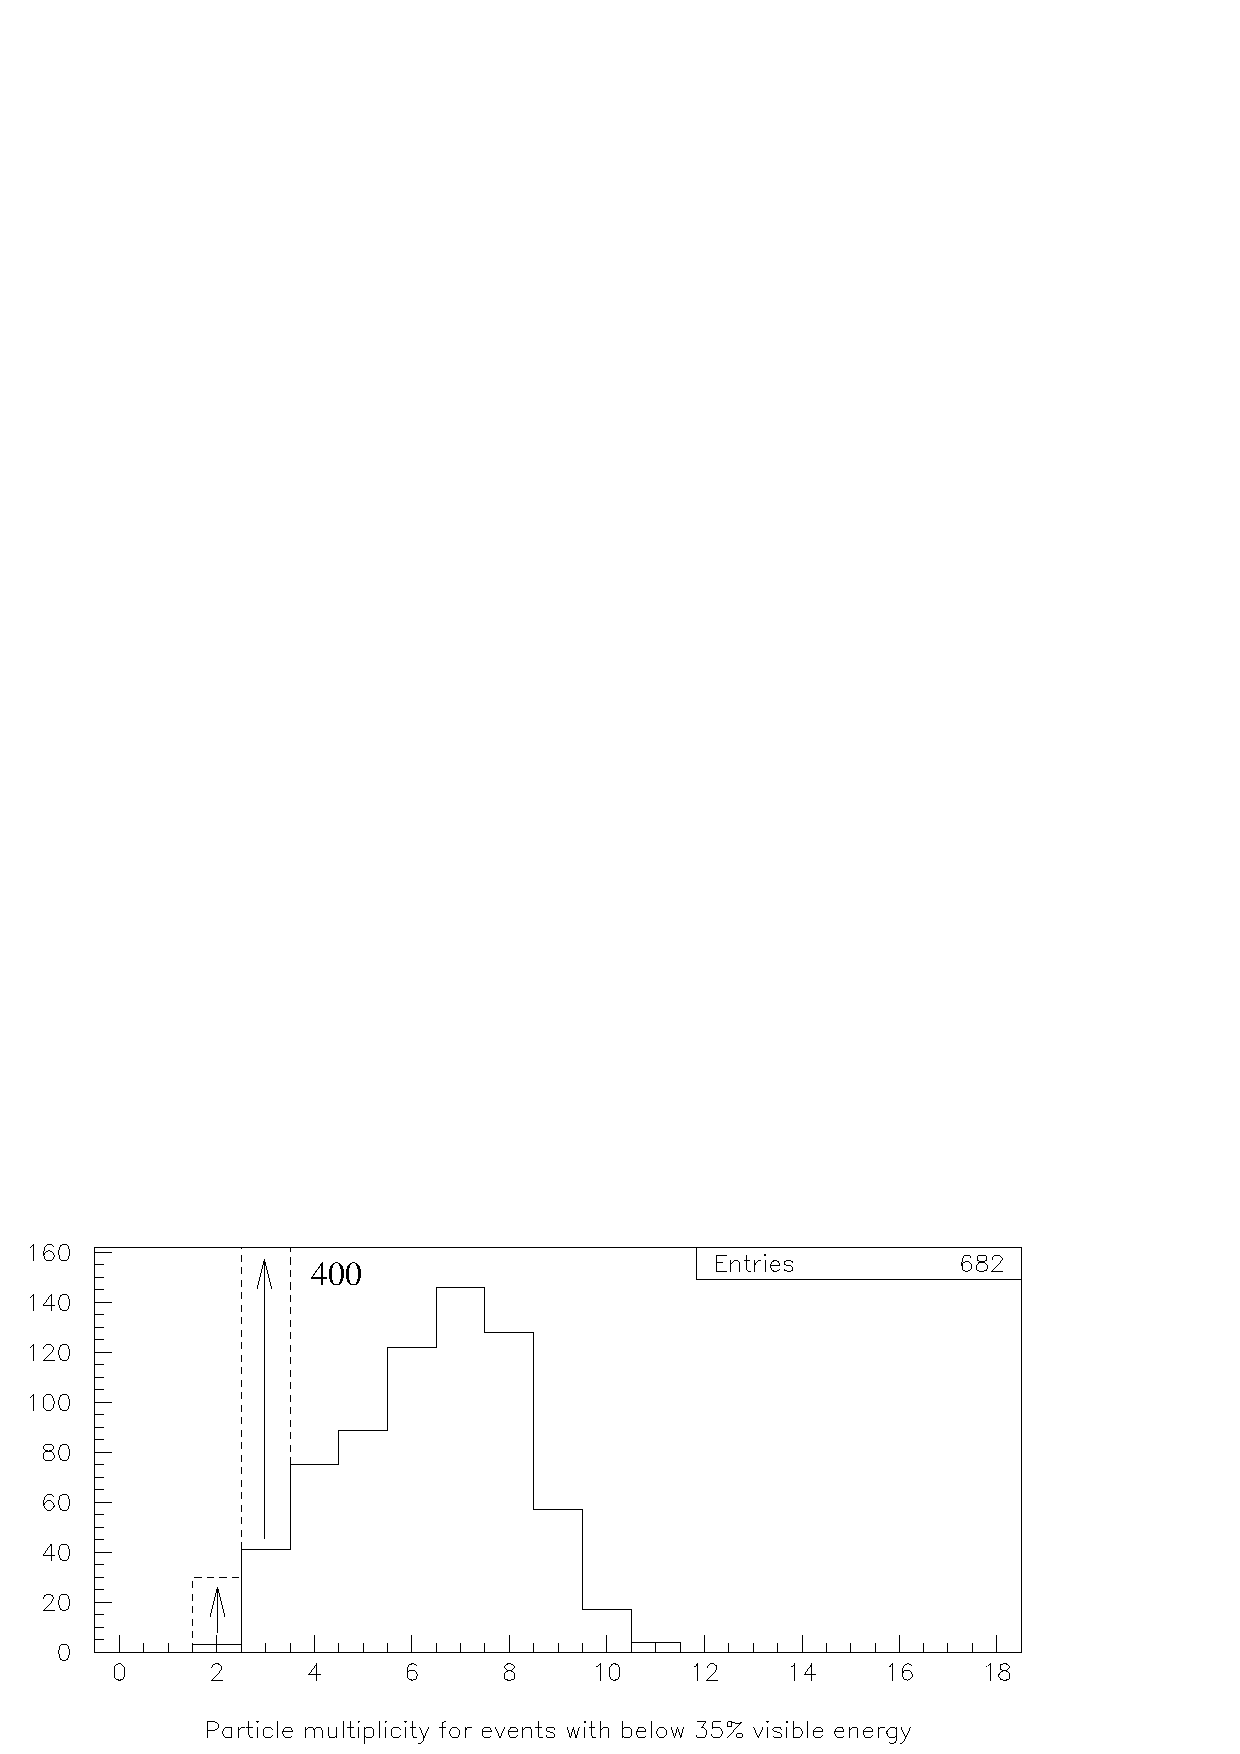
\includegraphics[width=\linewidth]{multiplicity_revamp.pdf}

\pagebreak

{\bf Example: Cut \# 6: Visible energy $>$ 35\% of center-of-mass energy}

\vfill

Uncertainty in detector response?  Simplify Monte Carlo so I can vary
parameters:

\begin{itemize}

  \item Event is divided into $N$ particles (average energy $\lambda$
  = 1.85 GeV / 10 GeV).

  \item A particle is lost with probability $p$ = 20\%.

  \item And reconstructed with $\Delta E$ = 120 MeV / 10 GeV.

\end{itemize}

(Agrees with data and Full Monte Carlo.)

\vfill

\includegraphics[width=\linewidth]{toymodel1_revamp.pdf}

\pagebreak

{\bf Example: Cut \# 6: Visible energy $>$ 35\% of center-of-mass energy}

\vfill

Vary parameters until Toy Model does not agree with data.

\vfill

Events that fail cut at most double.

\vfill

\includegraphics[width=\linewidth]{toymodel2_revamp.pdf}

\pagebreak

{\bf Example: Cut \# 6: Visible energy $>$ 35\% of center-of-mass energy}

\vfill

Vary parameters until Toy Model does not agree with data.

\vfill

Events that fail cut at most double.

\vfill

\includegraphics[width=\linewidth]{toymodel3_revamp.pdf}

\pagebreak

{\bf Example: Cut \# 6: Visible energy $>$ 35\% of center-of-mass energy}

\vfill

Vary parameters until Toy Model does not agree with data.

\vfill

Events that fail cut at most double.  $\Longrightarrow$ another 0.3\% uncertainty.

\vfill

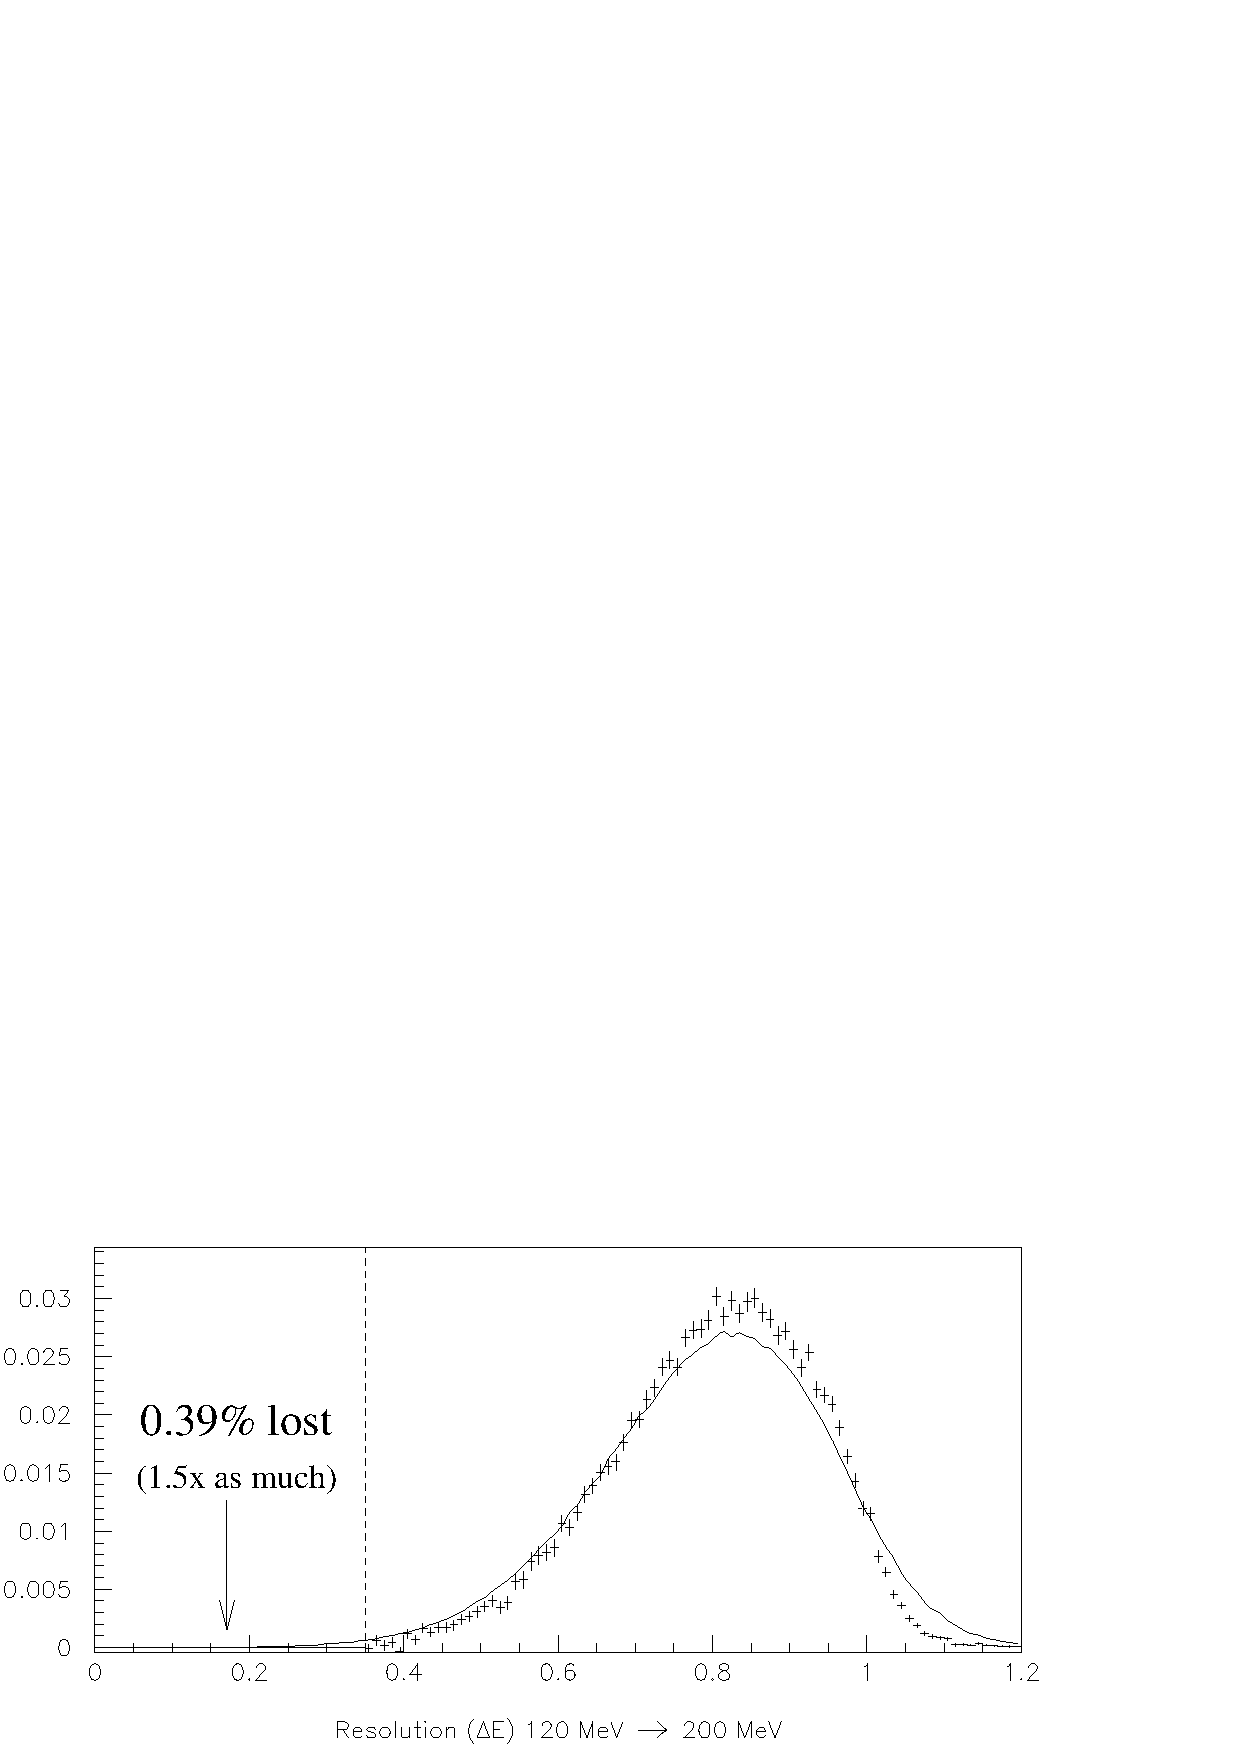
\includegraphics[width=\linewidth]{toymodel4_revamp.pdf}

\pagebreak

\begin{minipage}{\linewidth}

\begin{minipage}{0.22\linewidth}

\fbox{\begin{minipage}{\linewidth}

\begin{center}

\vspace{0.5 cm}

$\Upsilon(2S)$

\vspace{1 cm}

{\color{blue} squares} = MC \\
{\color{red} diamonds} = data

\vspace{0.5 cm}

\end{center}

\end{minipage}}

\vspace{8 cm}

\end{minipage}
\mbox{ } \mbox{ }
\begin{minipage}{0.76\linewidth}
  \includegraphics[height=\textheight]{cutbycut_2s_redux.pdf}
\end{minipage}

\end{minipage}

\pagebreak

\mbox{ }

\vspace{-\baselineskip}

\vfill

All $\Upsilon$s in CLEO-III have been counted on a run-by-run basis
with 1.5\% systematic errors.

%% \begin{center}
%%   \begin{tabular}{p{1 cm} c p{1 cm} c p{1 cm} c p{1 cm}}
%%     & $\Upsilon(1S)$ & & $\Upsilon(2S)$ & & $\Upsilon(3S)$ \\
%%     & 0.80\% & & 0.97\% & & 1.04\%
%%   \end{tabular} \mbox{\hspace{1 cm}}
%%   \begin{tabular}{c}
%%     \\
%%     systematic errors.
%%   \end{tabular}
%% \end{center}

\vfill

(Backgrounds and luminosity systematics have been given rough upper
limits of 0.5\% and 1.1\%, respectively.)

\vfill

{\tt http://www.lepp.cornell.edu/$\sim$mccann/upsilons\_in\_cleo3.dat}

{\tt http://www.lepp.cornell.edu/$\sim$mccann/upsilons\_in\_cleo3.explaination}

\vfill

\begin{center}
\begin{rotate}{90} \begin{minipage}{8 cm} \mbox{\hspace{2.5 cm}} Number of $\Upsilon$s \end{minipage} \end{rotate}
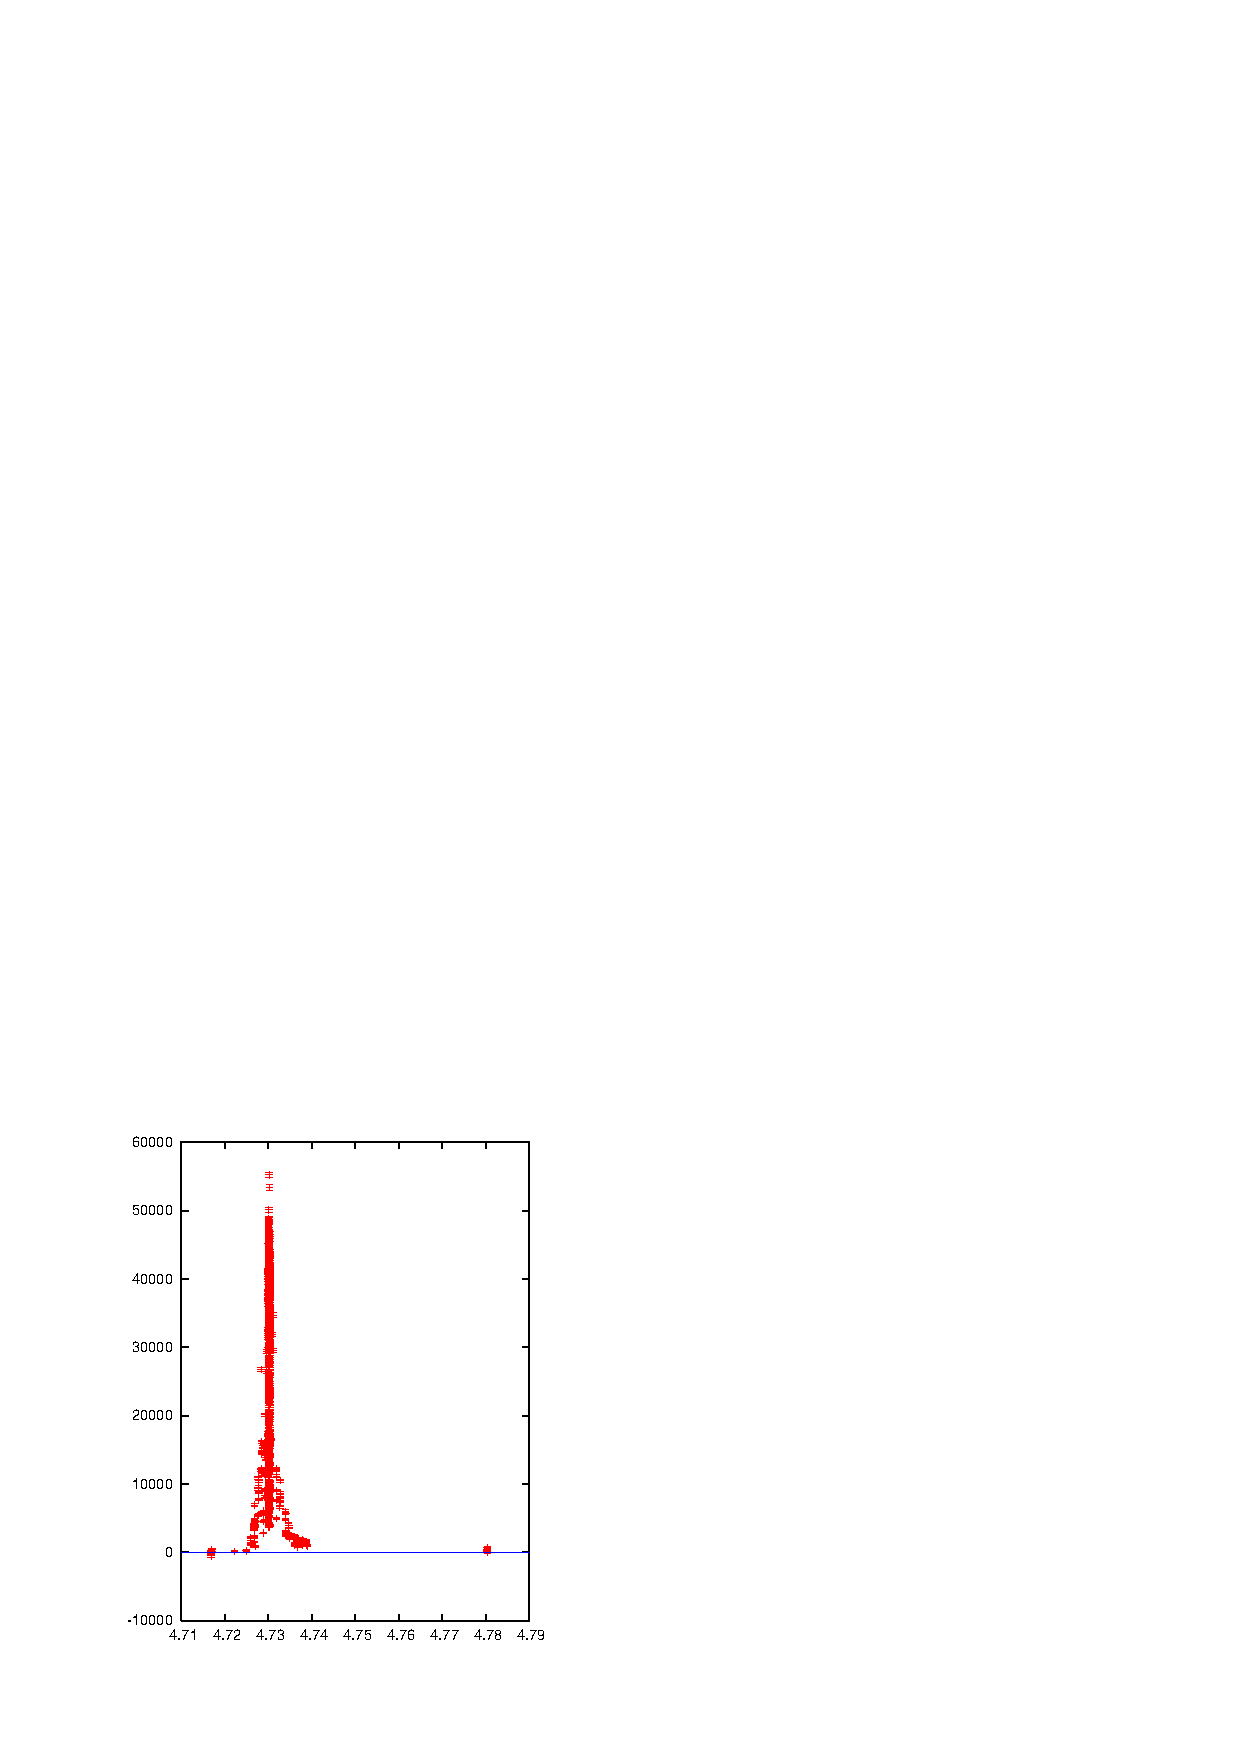
\includegraphics[width=0.3\linewidth]{plotme1.pdf}
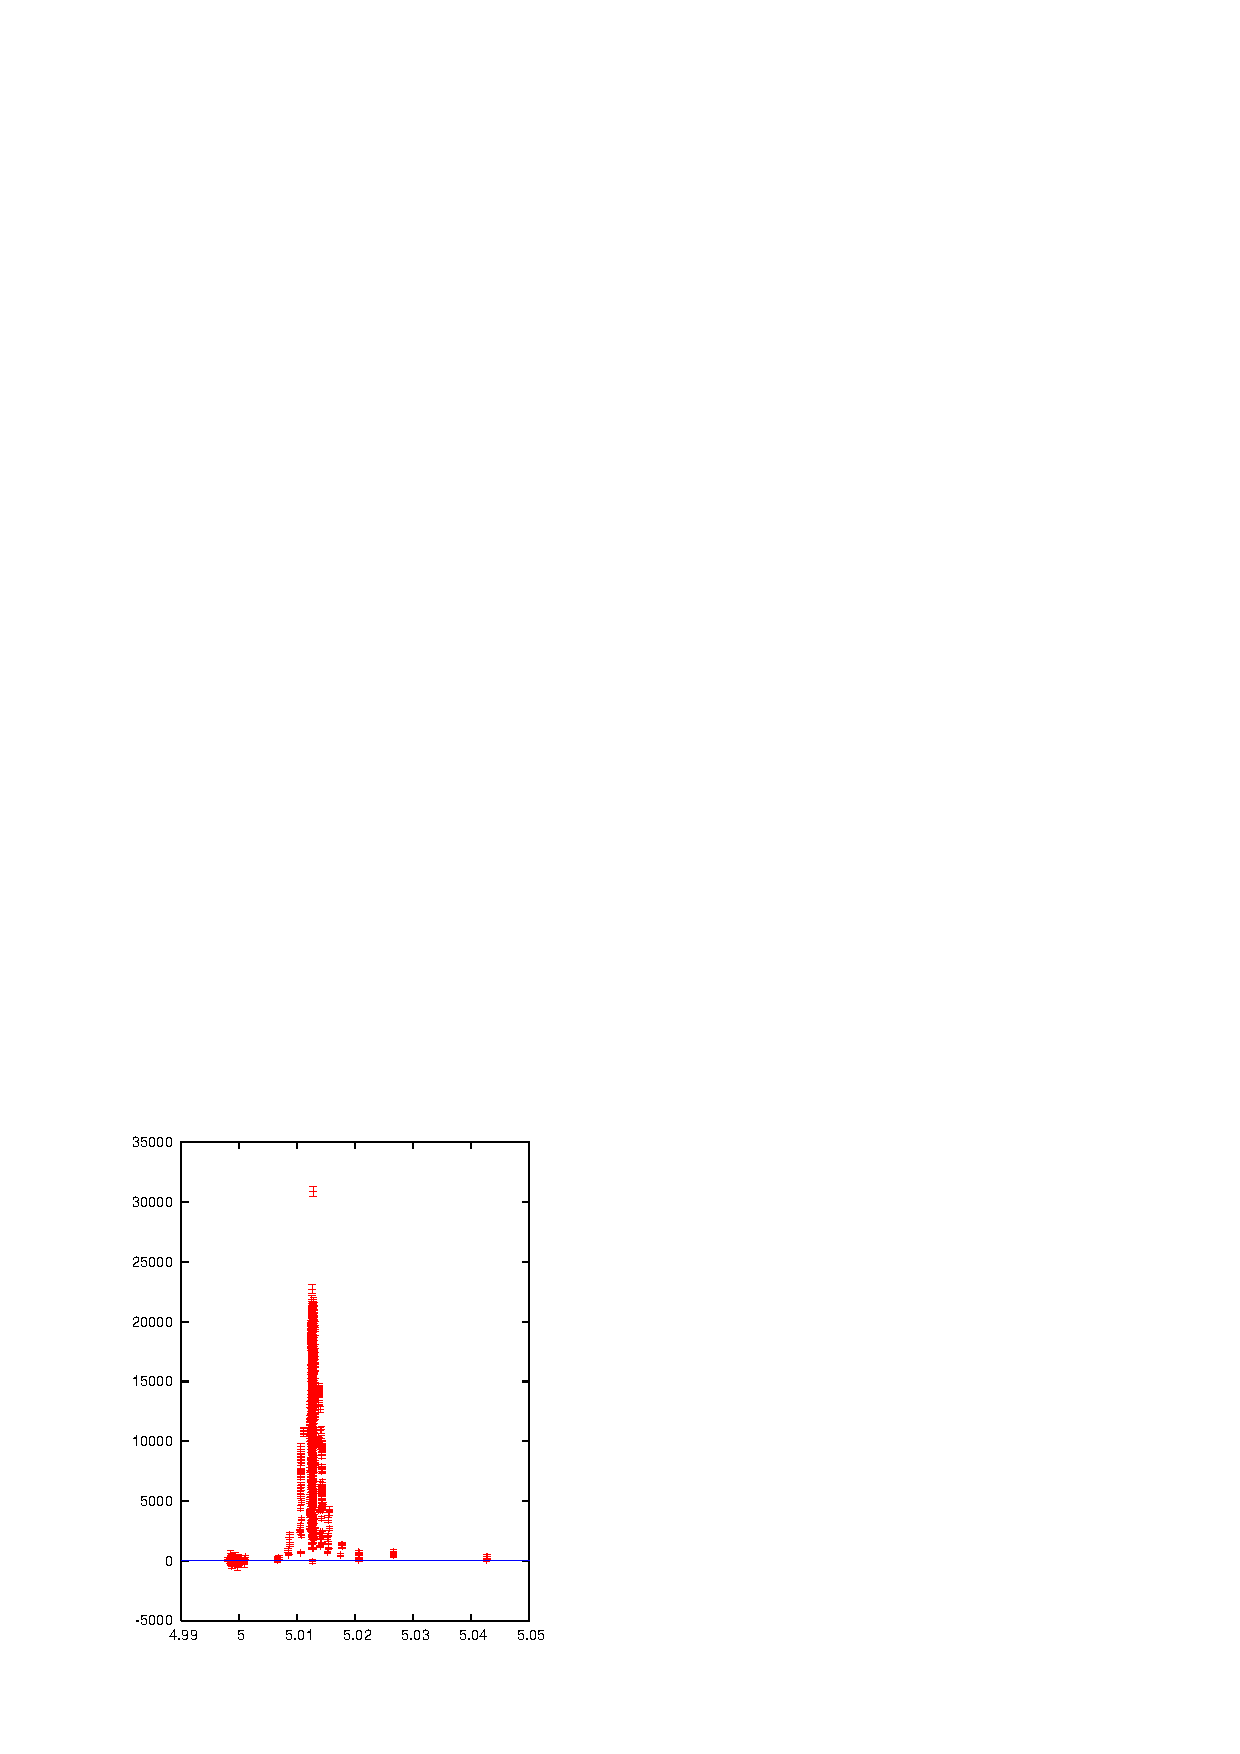
\includegraphics[width=0.3\linewidth]{plotme2.pdf}
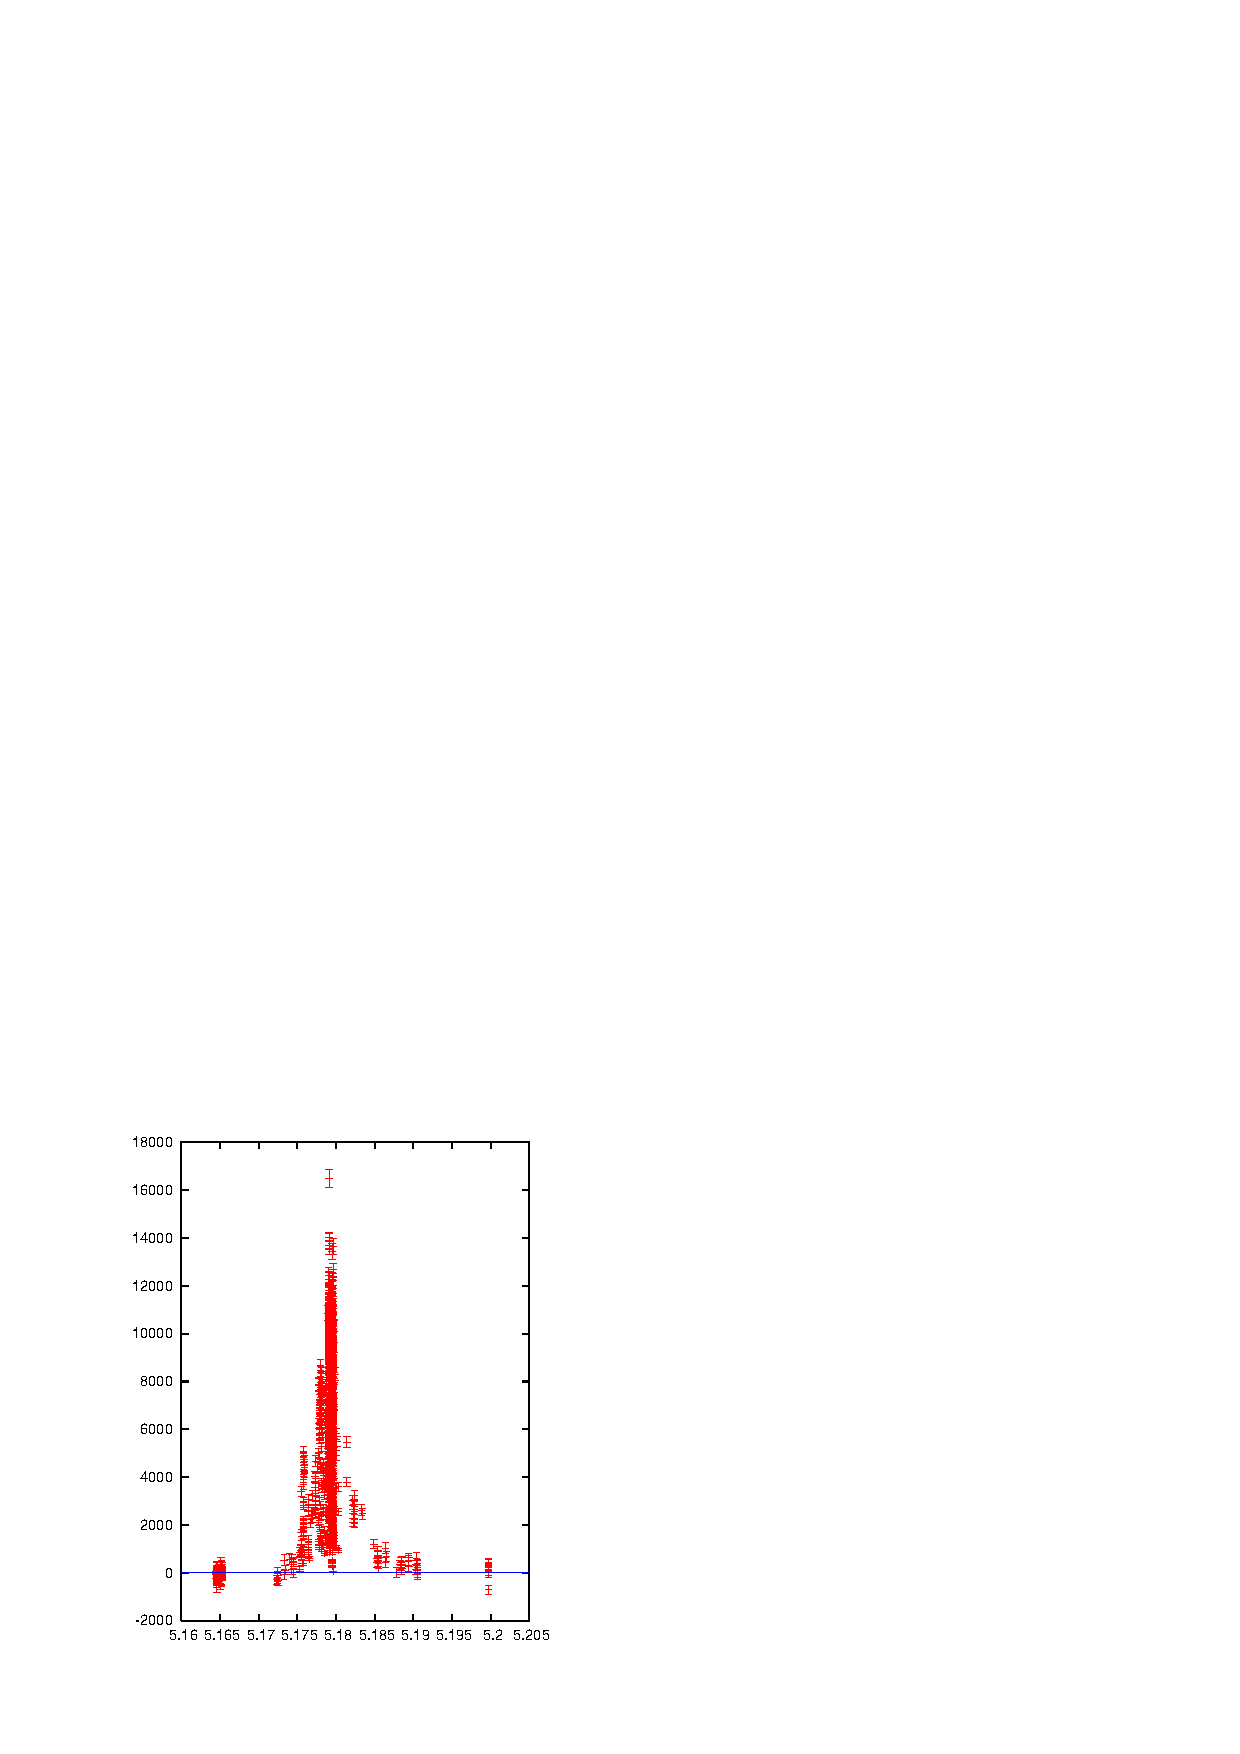
\includegraphics[width=0.3\linewidth]{plotme3.pdf}

Beam Energy (GeV)
\end{center}

\pagebreak

\mbox{ }

\vfill

\begin{center}\begin{minipage}{0.8\linewidth}

What's left for $\Gamma_{ee}$?

\vspace{1 cm}

\begin{enumerate}

  \item \sout{Lineshape Studies} 6 months

  \item \sout{Hadronic Efficiency} 2.75 years

  \item Backgrounds (with the new cuts) $\sim$ few weeks

  \item Luminosity \mbox{\hspace{0.5 cm}} $\gamma\gamma$-only: 3--6 months? \mbox{\hspace{0.5 cm}} bhabhas also: longer\ldots

  \item Beam energy stability: $<$ 1 month

\end{enumerate}

\end{minipage}\end{center}

\vfill

\fbox{\begin{minipage}{\linewidth} \Large $^*$This contains
forward-looking statements that are subject to risks, uncertainties
and other factors that could be deemed forward-looking and could cause
actual results to differ materially from those referred to in the
forward-looking statements. All statements other than statements of
historical fact are statements that could be deemed forward-looking
statements.
\end{minipage}}

\vfill

\mbox{ }

\end{document}
